% 电感
% 电感|法拉第|电磁感应|安培环路|感生电动势

\pentry{安培环路定理\upref{AmpLaw}, 法拉第电磁感应定律\upref{FaraEB}}

\textbf{电感器(inductor)}是电路中的一个元件, 当通过它的电流变化时, 它的两端会产生反向电动势从而抵抗电流的改变. 我们用物理量\textbf{电感}来描述电感器的这种性质的强弱, 记为 $L$, 定义如下
\begin{equation}
U = -L\dv{I}{t}
\end{equation}
也就是说反向电动势与电流的时间导数成正比, 比例系数就是电感.

\subsection{简单的电感模型}

\begin{figure}[ht]
\centering
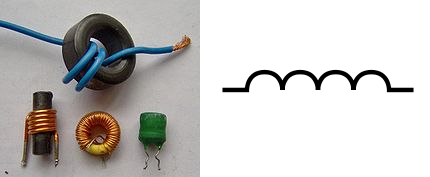
\includegraphics[width=9cm]{./figures/Induct_1.png}
\caption{左:各种电感器, 右:在电路图中的符号} \label{Induct_fig1}
\end{figure}
电感器的基本原理是利用线圈的自感, 即当线圈中有电流通过时, 会在它的内部及周围产生与电流大小成正比的磁场. 当电流发生改变时, 这个磁场也随之改变, 而根据法拉第电磁感应定律\upref{FaraEB}, 变化的磁场又会反过来作用在线圈上产生电动势.

由\autoref{AmpLaw_ex2}~\upref{AmpLaw}, 单位长度线圈数为 $n$, 长度为 $l$, 忽略边缘效应的螺线管, 内部磁场强度为
\begin{equation}
Bl = \mu_0nlI \Rightarrow B = \mu_0nI
\end{equation}
磁通量为
\begin{equation}
\Phi = BS = \mu_0nSI
\end{equation}
感生电动势为
\begin{equation}
U = -nL\dv{\Phi}{t} = -\mu_0n^2lS \dv{I}{t}
\end{equation}
令电感为
\begin{equation}\label{Induct_eq1}
L = \mu_0n^2lS
\end{equation}
有
\begin{equation}
U = -L\dv{I}{t}
\end{equation}

\subsection{电感储存的能量}
与电容类似, 电感器中也可以储存能量.
\begin{equation}
E_B = \frac{1}{2}L I^2
\end{equation}

\subsubsection{推导}
\begin{equation}
E_B = -\int_0^{I_m} U I \dd{t} = \int_0^{I_m} L \dv{I}{t} I \dd{t} = L\int_0^{I_m} I \dd{I} = \frac{1}{2} L I^2
\end{equation}
